\chapter{Implementacja}
\label{cha:implementacja}

tutaj gadane jakiś ogólny opis i w ogóle cnie

%---------------------------------------------------------------------------

\section{Wybór technologii}

%---------------------------------------------------------------------------

\section{Wielowątkowe tworzenie ofert}

%---------------------------------------------------------------------------

\section{Autoryzacja użytkownika w Allegro}

Do integracji serwisu z aplikacją potrzebne jest pozyskanie tokenu dostępowego. Allegro udostępnia tzw. ``ścieżkę device flow``, dzięki której cały proces odbywa się bez konieczności uwzględniania go w interfejsie graficznym. Poniżej zaprezentowany jest diagram prezentujący tę funkcjonalność.\\

\begin{figure}[H]
	\centering
	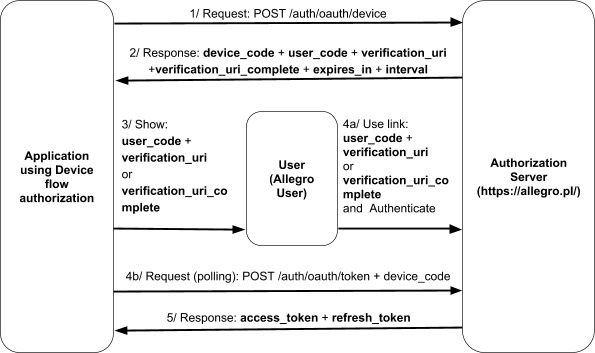
\includegraphics[width=\linewidth]{device_flow.png}
	\caption{Autoryzacja użytkownika typu Device flow}
	\caption*{Źródło: {https://developer.allegro.pl/}}
\end{figure}

Podejście w tej pracy zakłada zarejestrowanie jednego, wspólnego dla całego systemu, konta funkcjonalnego za pomocą którego każde zapytanie będzie autentykowane. Stwarza to niestety jedno ograniczenie, a mianowicie, ze względu na obowiązujący główny limit nakładany na Client ID po przekroczeniu liczby 9000 zapytań na minutę, aplikacja zwróci status HTTP 429 i zostanie zabklokowana na kolejne 60 sekund.\\
W fazie inicjalizacyjnej autoryzacji uzyskane zostaną dwa unikalne tokeny: 
\begin{itemize}
	\item dostępowy - ważny przez 12h.
	\item odświeżający - ważny 6 miesięcy.
\end{itemize}
Zostaną one zachowanie w pamięci, a każde kolejne zapytanie, w przypadku wygaśnięcia tokenu dostępowego, spowoduje jego odnowienie.
\begin{figure}[H]
	\centering
	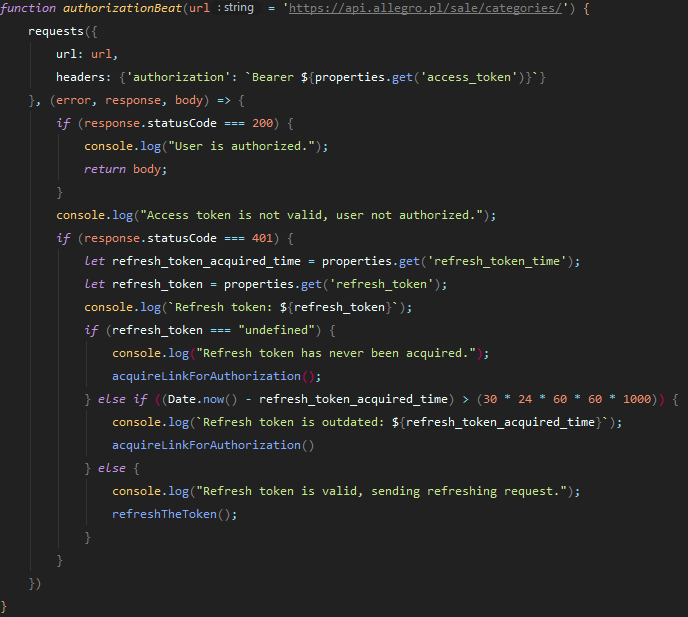
\includegraphics[width=\linewidth]{authorization.png}
	\caption{Kod odpowiedzialny za utrzymywanie ważnego tokena}
\end{figure}
Powyższy kod prezentuje przebieg akcji, które maja miejsce za każdym razem, kiedy otrzymywane jest zapytanie do OffersService(2.4). Na początku sprawdzane jest, czy token jest zwyczajnie aktualny, następnie, w przypadku, gdy nie jest, pobierany jest token odświeżający. W zależności od tego, czy jest on ważny, wygaśnięty, czy może w ogóle nigdy nie został uzyskany, odpowiednia logika zostaje uruchomiona.

%---------------------------------------------------------------------------


\section{Wdrożenie}

%---------------------------------------------------------------------------

\section{Elementy konifguracyjne}

%---------------------------------------------------------------------------